\documentclass{beamer}
\mode<presentation>
\usepackage{amsmath}
\usepackage{amssymb}
\usepackage{bm}
\usepackage{adjustbox}
\usepackage{subcaption}
\usepackage{enumerate}
\usepackage{multicol}
\usepackage{mathtools}
\usepackage{listings}
\usepackage{url}
\def\UrlBreaks{\do\/\do-}
\usetheme{Boadilla}
\usecolortheme{lily}
\setbeamertemplate{footline}
{
  \leavevmode%
  \hbox{%
  \begin{beamercolorbox}[wd=\paperwidth,ht=2.25ex,dp=1ex,right]{author in head/foot}%
    \insertframenumber{} / \inserttotalframenumber\hspace*{2ex} 
  \end{beamercolorbox}}%
  \vskip0pt%
}
\setbeamertemplate{navigation symbols}{}

\providecommand{\nCr}[2]{\,^{#1}C_{#2}}
\providecommand{\nPr}[2]{\,^{#1}P_{#2}}
\providecommand{\mbf}{\mathbf}
\providecommand{\pr}[1]{\ensuremath{\Pr\left(#1\right)}}
\providecommand{\qfunc}[1]{\ensuremath{Q\left(#1\right)}}
\providecommand{\sbrak}[1]{\ensuremath{{}\left[#1\right]}}
\providecommand{\lsbrak}[1]{\ensuremath{{}\left[#1\right.}}
\providecommand{\rsbrak}[1]{\ensuremath{\left.#1\right]}}
\providecommand{\brak}[1]{\ensuremath{\left(#1\right)}}
\providecommand{\lbrak}[1]{\ensuremath{\left(#1\right.}}
\providecommand{\rbrak}[1]{\ensuremath{\left.#1\right)}}
\providecommand{\cbrak}[1]{\ensuremath{\left\{#1\right\}}}
\providecommand{\lcbrak}[1]{\ensuremath{\left\{#1\right.}}
\providecommand{\rcbrak}[1]{\ensuremath{\left.#1\right\}}}
\providecommand{\rank}{\text{rank}}
\theoremstyle{remark}
\newtheorem{rem}{Remark}
\newcommand{\sgn}{\mathop{\mathrm{sgn}}}
\providecommand{\abs}[1]{\ensuremath{\left\vert #1 \right\vert}}
\providecommand{\res}[1]{\Res\displaylimits_{#1}} 
\providecommand{\norm}[1]{\lVert#1\rVert}
\providecommand{\mtx}[1]{\mathbf{#1}}
\providecommand{\mean}[1]{\overline{#1}}
\providecommand{\fourier}{\overset{\mathcal{F}}{ \rightleftharpoons}}
\providecommand{\system}{\overset{\mathcal{H}}{ \longleftrightarrow}}
\providecommand{\dec}[2]{\ensuremath{\overset{#1}{\underset{#2}{\gtrless}}}}

% this \vec is already defined in your file:
\renewcommand{\vec}[1]{\begin{pmatrix}#1\end{pmatrix}}

\newenvironment{amatrix}[1]{%
  \left(\begin{array}{@{}*{#1}{c}|c@{}}
}{%
  \end{array}\right)
}

\lstset{
frame=single, 
breaklines=true,
columns=fullflexible
}
\usepackage{listings}
\lstset{
  language=Python,
  basicstyle=\ttfamily\small,
  numbers=left,
  numberstyle=\tiny,
  breaklines=true,
  frame=single
}

\title{Matgeo-4.4.15}
\author{AI25BTECH11019-Menavath Sai Sanjana}

\date{}

\begin{document}

\begin{frame}
\titlepage
\end{frame}

\begin{frame}
\frametitle{Question}
Find the sum of the intercepts cut off by the plane  
$-\vec{r}\cdot(2\hat{i}+\hat{j}-\hat{k})-5=0$ on the three coordinate axes.  
\end{frame}

\begin{frame}
\frametitle{Solution}
The given plane is
\begin{align}
-\vec{r}\cdot\vec{2\\1\\-1}-5=0 
&\implies \vec{r}\cdot\vec{2\\1\\-1}+5=0
\end{align}

\textbf{X-intercept:} $(x,0,0)$  
\begin{align}
\vec{r}=\vec{x\\0\\0},\quad 
\vec{r}\cdot\vec{2\\1\\-1}+5=0 
&\implies 2x+5=0 \\
x&=-\frac{5}{2}
\end{align}

\textbf{Y-intercept:} $(0,y,0)$  
\begin{align}
\vec{r}=\vec{0\\y\\0},\quad 
\vec{r}\cdot\vec{2\\1\\-1}+5=0 
&\implies y+5=0 \\
y&=-5
\end{align}
\end{frame}

\begin{frame}
\frametitle{Solution(Continuation)}
\textbf{Z-intercept:} $(0,0,z)$  
\begin{align}
\vec{r}=\vec{0\\0\\z},\quad 
\vec{r}\cdot\vec{2\\1\\-1}+5=0 
&\implies -z+5=0 \\
z&=5
\end{align}

\end{frame}

\begin{frame}
\frametitle{Conclusion}
\noindent\textbf{Conclusion:}  
The intercepts cut off are
$
x=-\frac{5}{2},\;
y=-5,\;
z=5.
$  

Hence, the sum of intercepts is  
$
-\frac{5}{2} - 5 + 5 \;=\; -\frac{5}{2}.
$
\end{frame}

\begin{frame}
\frametitle{Graphical Representation}

\begin{figure}[ht!]
    \centering
    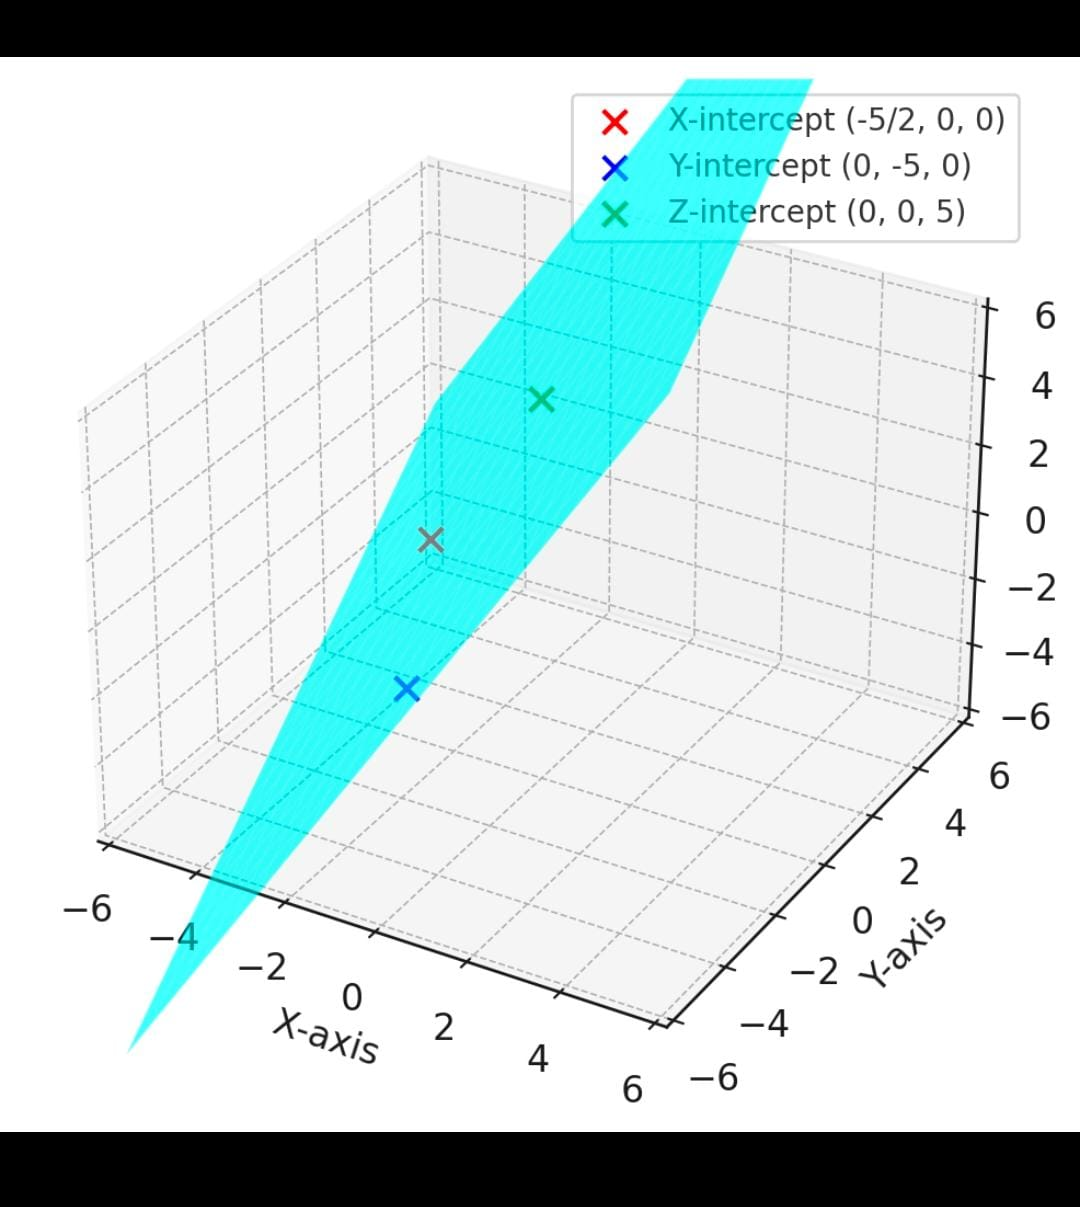
\includegraphics[width=0.65\textwidth]{matgeo-4.4.15.jpeg}
    \caption{}
    \label{fig:triangle5cm}
\end{figure}
\end{frame}

\end{document}
